\chapter{Webserver und dessen Integration in CYBOI}

  \section{Hintergrund}
  
    
    Zur Beantwortung einer Anfrage eines Clients an einen Server �ber das  
    Http-Protokoll ist ein Webserver n�tig.
    Dies kann durch einen vorhandenen Webserver, wie z.B. Apache, oder durch einen selbst 
    programmierten Webserver realisiert werden. Dieser Webserver muss f�r CYBOL
    angepasst werden. Bei einem bestehenden Webserver ist eine Erweiterung 
    z.B. durch ein CYBOI-Plugin m�glich. Der Vorteil der Erweiterung eines bestehenden Webservers
    ist die Verwendung der ganzen Funktionalit�t, wie z.B. die Session-Verwaltung und 
    die Skalierbarkeit. Das Hauptproblem bei der Integration
    w�re die Anpassung der verschiedenen Softwarearchitekturen (bestehender Webserver und CYBOI).   
    Ein weiterer Nachteil ist die Abh�ngigkeit des Plugins zu einem bestehenden 
    Webserver, das bedeutet dass bei �nderungen des Webservers auch das Plugin anzupassen ist.
    Die Kontrolle w�rde nicht allein beim CYBOP-Projekt liegen. 

    Da die Implementierung f�r CYBOL insgesamt als Prototyp geplant ist, reicht es aus,
    einen kleinen Webserver selbst zu programmieren, so dass man 
    die gesamte Verf�gungsgewalt �ber das Projekt 
    und dessen Quelltext hat. Weiterhin kann im Softwaredesign eine bessere Homogenit�t erreicht werden.
    �nderungen am Webserver sind somit leichter zu realisieren. Der Nachteil ist hier, das die
    Standardfunktionalit�t von Webservern, wie z.B. die Session-Verwaltung, in CYBOI 
    programmiert werden muss. 
    
    Die Vorraussetzungen f�r einen Webserver sind die Sockets. Diese stellen die 
    Kommunikationsschnittstelle zwischen den einzelnen Komponenten dar. Wichtiger 
    Bestandteile f�r die Integration des Webserver-Prototyps in CYBOI
    sind Prozesse und Threads. Da bei der Implementierung der Sockets blockierende
    Sockets verwendet werden, 
    %\(siehe Abschnitt ref{{blocksocktets}), 
    ist es notwendig
    den Webserver in einem eigenen Prozess bzw. Thread laufen zu lassen. 
    
      \section{Sockets}  
  
     Sockets sind nach \cite{defsockets} folgenderma�en definiert. 
    \begin{quotation}
      Sockets is a method for communication between a client program and a server program in a network. 
      A socket is defined as the endpoint in a connection. Sockets are created and used with a set 
      of programming requests or function calls sometimes called the sockets application 
      programming interface (API). The most common sockets API is the Berkeley UNIX C language 
      interface for sockets. Sockets can also be used for communication between processes 
      within the same computer. 
    \end{quotation}
    
    Ein Socket ist also eine Schnittstelle zwischen einem Prozess 
    und einem Transportprotokoll. Letzteres kann z.B. TCP oder UDP sein. 
    Das Socket-Prinzip entspricht dem von File-Deskriptoren. 
    Dort repr�sentiert nach dem �ffnen einer Datei ein Handle die Verbindung
    zu dieser Datei und unter Angabe des Handles ist der Lese- oder Schreibzugriff m�glich. 
    Bei Sockets geht es jedoch nicht um physikalische Dateien sondern um Kommunikationskan�le, �ber 
    die Daten gesendet und empfangen werden k�nnen.

    Socket-Schnittstellen sind zwar von keiner Institution genormt, 
    stellen aber einen de-facto- bzw. Industriestandard dar, was zum einen daran liegen d�rfte, 
    dass sie leicht verst�ndlich sind, zum anderen f�gen sie sich ausgesprochen 
    harmonisch in die UNIX-Umwelt ein. Eine Variante der Socket-Schnittstelle wurde von 
    Microsoft und verschiedenen anderen Firmen unter der Bezeichnung WinSock in das 
    Schnittstellenangebot der Windows Open Service Architecture (WOSA) aufgenommen und 
    d�rfte damit auch ein etablierter Standard in der PC-Welt sein.
    
    \subsection{Arten von Sockets}
    
      Sockets stellen eine allgemeine Form der Kommunikation zwischen Dateien, Prozessen usw. dar.
      Schon allein die Verwendung unterschiedlicher �bertragungsprotokolle 
      spezifiziert unterschiedliche Anwendungsgebiete. 
      Folgende Arten von Sockets werden darum unterschieden:
      
      \begin{itemize}
        \item Stream Socket \\
              Stream Sockets setzen auf dem verbindungsorientierten TCP auf. Er ist
              langsamer als ein Datagramm Socket, aber daf�r wird die �bertragungskontrolle 
              gew�hrleistet.
        \item Datagram Socket \\
              Datagram Sockets setzen auf dem verbindungslos orientierten User Datagram Protocol (UDP) auf.
              Das gro�e Problem dabei ist, dass die �bertragungskontrolle fehlt. Ansonsten ist die 
              �bertragungsart sehr schnell, falls die Pakete ankommen und erzeugt kaum
              Overhead.
        \item Raw Socket \\
              Ein Raw Socket ist ein spezieller Socket. Er erm�glicht dem Benutzer den 
              direkten Zugang zum Netzwerk, 
              indem man eigene Pakete einspeisen kann. Raw Socket benutzen z.B. das Protokoll ICMP. 
              Sie sind sehr 
              schnell, da sie auf eine tiefere Protokollfamilie aufsetzen und damit weniger Overhead haben. 
        \item Unix Domain Sockets \\
              Unix verwendet Sockets zur lokalen Interprozess-Kommunikation, sog. Unix Domain Sockets. 
              Sie sind Teil des POSIX-Standards. Dies ist die urspr�ngliche Form des 
              von BDS entwickelten Sockets.
      \end{itemize}
  
      F�r den Webserver der vorliegenden Diplomarbeit wird ein Stream Socket mit dem Protokoll TCP verwendet.  
      Da in einer Anwendung sichergestellt werden muss, das die Datenpakete ankommen und 
      auch in der richtigen Reihenfolge zusammengesetzt werden, ist nur ein Stream Socket mit der 
      entsprechenden �bertragungskontrolle verwendbar.

    \subsection{Arbeitsweise von Sockets}
    
      Sockets arbeiten immer nach einen bestimmten Muster. Als erstes ist der Server f�r die
      Bearbeitung des Sockets vorzubereiten. Dazu muss er veranlasst werden �ber einen bestimmten
      Port auf die Anforderungen der Clients zu warten. Ports geh�ren zu der Adresskomponente 
      einer Netzwerkkommunikation. Der Port ist mit 16 Bit kodiert. Damit kann der Port Werte von 
      0 bis 65535 annehmen. Die Ports bis zur 1024 sind f�r verschiedenen Dienste (FTP, HTTP, ...)
      definiert. Die Portnummern h�her als 1024 stehen zur freien Verf�gung, wobei sich auch hier schon
      f�r gewisse Dienste  Standard-Portnummern eingeb�rgert haben. 
      
      In der Abbildung \ref{fig:tcpsocket} ist einen typischen Ablauf eines Stream Sockets zu sehen.
      \begin{figure}[H]
        \centering
          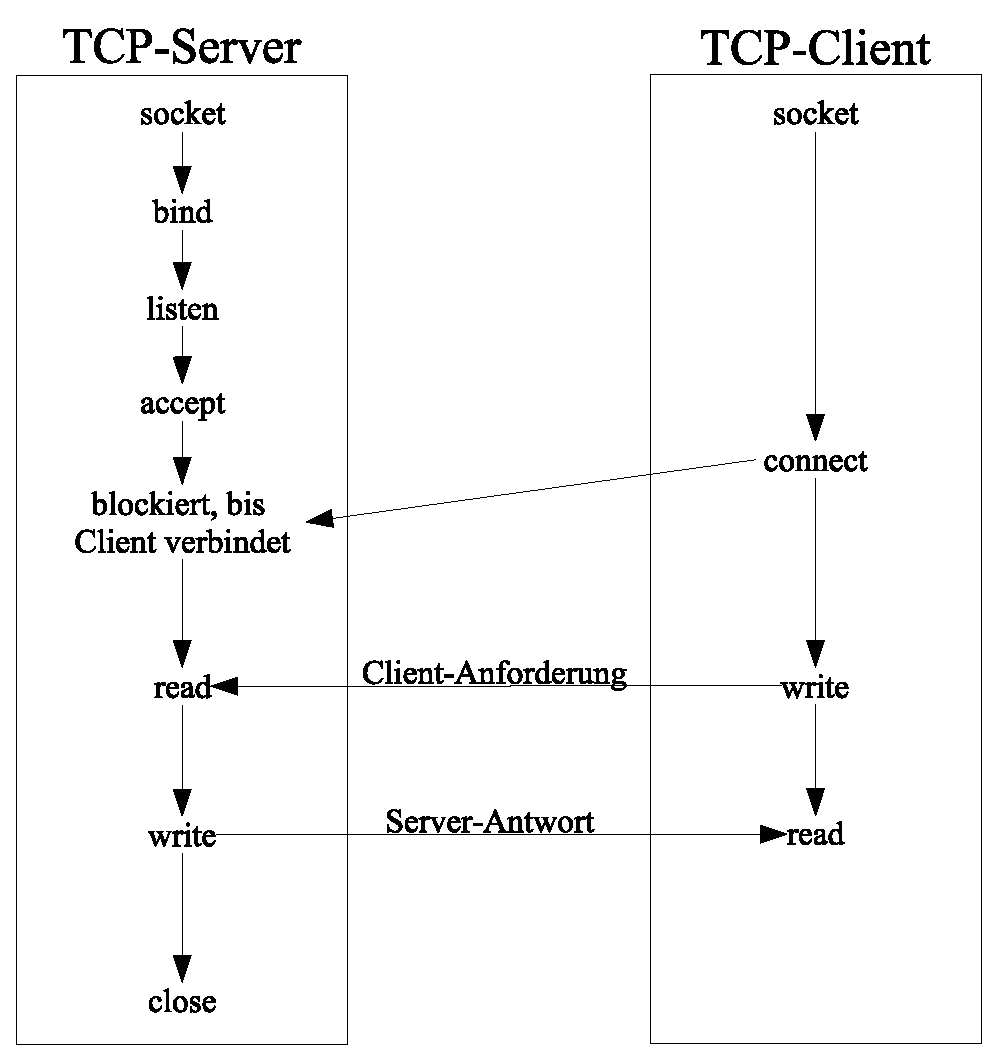
\includegraphics[width=10cm]{images/tcpsocket.eps}
        \caption{Ablauf TCP-Socket}
        \label{fig:tcpsocket}
      \end{figure}
      Als erstes muss der Socket erstellt werden. Mit \emph{bind} wird dieser Socket 
      an eine bestimmte Portnummer gebunden und mit dem Befehl \emph{listen} wird 
      dem Socket mitgeteilt, das er auf Verbindungsversuche zu dieser Portnummer 
      lauschen soll. Jetzt wartet der Server mit \emph{acceppt} auf einen 
      Verbindungsversuch des Clients. Dies ist entweder als blockierende oder
      nicht blockierende Funktion implementiert (siehe Abschnitt \ref{blocksocktets}). 
      Nach dem \emph{accept} die Verbindung akzeptiert hat, wird der normale
      Kommunikationsprozess durchgef�hrt. Als erstes liest der Server (\emph{read}) die Anfrage
      vom Client und schickt eine Antwort (\emph{write}) an den Client zur�ck.
      Danach ist vom Server die Verbindung zu beenden (\emph{close}).


    \subsection{Blockierende und nicht blockierende Sockets}
      \label{blocksocktets}  
  
      Gewisse Funktionen einer Socketoperation k�nnen als blockierende oder nicht blockierende 
      Operation ausgef�hrt werden. Blockierend bedeutet, dass die Funktion so lange wartet,
      d.h. dass das restliche Programm an dieser Stelle unterbrochen wird, 
      bis die Aktion ausgef�hrt wurde. Eine typische Operation ist das Warten auf eine
      Anfrage vom Client. In dieser Zeit ist der Prozess stillgelegt, bis eine Anfrage 
      auf dem Kommunikationskanal anliegt. So lange der Prozess wartet, wird keine
      Prozessorleistung verbraucht. Andere Prozesse auf 
      dem Rechner k�nnen normal weiterarbeiten, da der Prozessor keine Belastung durch das
      Warten auf eine Anfrage hat. Wenn diese Operation als nicht blockierende 
      Operation realisiert w�re, so w�rde, wenn kein Anfragesignal auf dem 
      Kommunikationskanal anliegt, die Funktion an dieser Stelle nicht warten, sondern einfach 
      im Programm weitermachen. Um nun eine Anfrage �ber das Socket zu registrieren, ist die Ausf�hrung 
      der Operation in einer Endlosschleife n�tig. Dies verbraucht aber viele Ressourcen des Prozessors.
      Auf Grund der Performance des Gesamtsystems sind also blockierende Sockets vorzuziehen.

    
    \section{Prozesse und Threads}

  Da die Implementierung des Webservers mit blockierenden Sockets erfolgt, ist
  es erforderlich, parallele bzw. nebenl�ufige Programme in CYBOI zu starten, 
  da ansonsten die blockierenden Socketoperationen den gesamten
  Interpreter CYBOI lahm legen. Es gibt zwei M�glichkeiten parallele bzw. nebenl�ufige 
  Programme zu starten, entweder als eigenst�ndiger Prozess oder 
  als Thread. F�r die Auswahl sind beide Varianten zu erkl�ren und Vor- und Nachteile 
  gegen�berzustellen. 
     
  \subsection{Prozess}
   
    Ein Prozess aus Betriebssystemsicht ist ein in Ausf�hrung befindliches Programm,
    welches sequentiell abgearbeitet wird. Es wird immer nur
    eine Instruktion zu einer bestimmten Zeit ausgef�hrt. Ein Prozess besteht
    aus dem Programm und der Programmumgebung und er verf�gt �ber einen
    eigenen Adressraum. Zu der Programmumgebung geh�ren Programmz�hler, 
    alle Registerinhalte, Stack (tempor�re Daten) und der Datenbereich (globale Variablen).
    Da das Betriebssystem mehrere Prozesse
    gleichzeitig verwaltet und es so aussieht, als ob die Prozesse parallel ablaufen, 
    m�ssen diese Prozesse verschieden Zust�nde annehmen k�nnen. Folgendes Bild veranschaulicht die
    Prozesszust�nde und welche Wechsel zwischen den Prozesszust�nden m�glich sind.
  
    \begin{figure}[H]
      \centering
        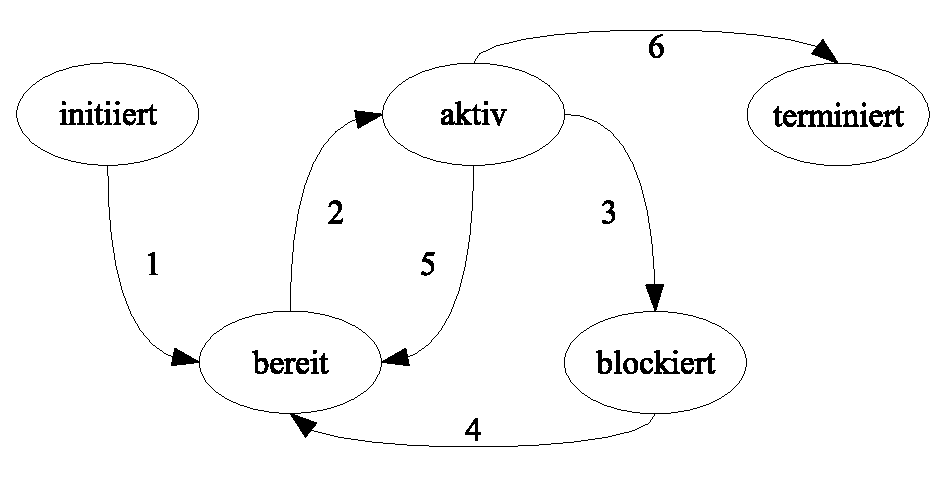
\includegraphics{images/prozeszustaende.eps}
      \caption{Prozesszust�nde}
      \label{fig:prozeszustaende}
    \end{figure}

    Als erstes wird ein Prozess initiiert. Dazu werden alle Initialbetriebsmittel
    alloziiert (1). Danach ist der Prozess in dem Zustand \emph{bereit}. In diesem Zustand kann der Prozess
    noch nichts machen, da ihm noch keine Prozessorzeit zugeordnet ist. Dies wird durch
    den Prozessscheduler des Betriebssystems realisiert (2). Dieser Scheduler kann den Prozess
    auch wieder in den Zustand \emph{bereit} zur�ckversetzen (5). Dies kann z.B. durch Ablauf der Zeitscheibe 
    oder durch Priorit�tensteuerung passieren. Wird von einem aktiven Prozess ein
    Betriebsmittel angefordert und dieses ist zurzeit nicht verf�gbar, so wird der Prozess 
    in den Zustand blockiert gesetzt (3). Liegt ein Signal an, dass das erwartete Betriebsmittel 
    zur Verf�gung steht,
    so wechselt der Status des Prozesses in den Zustand \emph{bereit} (4).
    Am Ende wird der Prozess abgeschlossen und alle Betriebsmittel und Ressourcen werden freigegeben. 
    
    Um zwischen den Prozessen umschalten zu k�nnen, m�ssen Informationen des Prozesses gesichert werden.
    Dazu dienen so genannte Prozess-Kontroll-Bl�cke (PKB). Diese beinhalten folgende Informationen:
    \begin{itemize}
      \item Prozesszustand
      \item Zeiger auf Prozess
      \item Prozess-Id
      \item Programmumgebung
      \begin{itemize}
        \item Programmz�hler
        \item Prozessorregister
        \item I\/O Statusinformationen
         \item Speicherverwaltungsinformationen
      \end{itemize}
    \end{itemize}
    Um nun von einen zum anderen Prozess zu wechseln, wird der gesamte PKB gesichert 
    und der PKB vom aktivierten Prozess geladen. Diese Art von Prozessen wird auch als 
    Single-Thread-Prozessor-Modell bezeichnet.
    \begin{figure}[H]
      \centering
        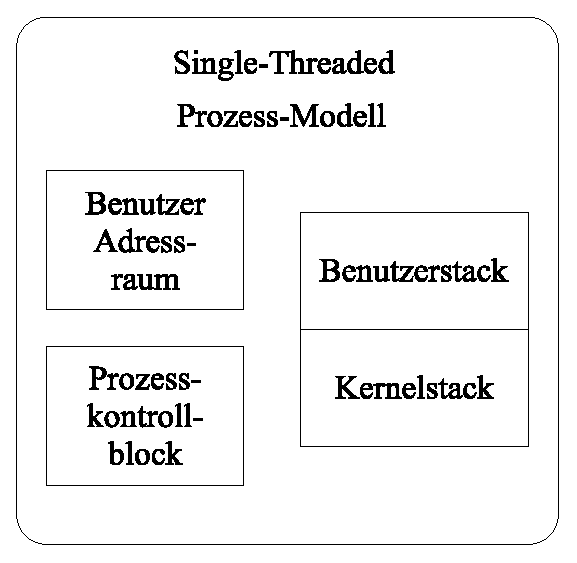
\includegraphics{images/singlethreadprozess.eps}
      \caption{Single-Thread-Prozess-Modell}
      \label{fig:singlethreadprozess}
    \end{figure}
    
   Ein Prozess kann weitere Unterprozesse
   generieren, so dass eine Baumstruktur von Prozessen und ihren Unterprozessen
   entsteht. Die Umschaltung zwischen den Prozessen (siehe vorheriges Kapitel) erfordert
   die Sicherung und das Laden des gesamten Prozess-Kontroll-Block und der Stacks. 
   
  \subsection{Parallele und nebenl�ufige Prozesse}
  
   Ein Prozess wird sequentiell im Prozessor abgearbeitet. Richtige parallele
   Arbeitung von Prozessen gibt es nur in Mehrprozessorrechnern. In 
   Einprozessormaschinen gibt es keine echte parallele Verarbeitung, sondern
   nur eine nebenl�ufige (quasi parallel) Abarbeitung von Prozessen. 
   Dies wird durch das Betriebssystem intern geregelt. 
   Da es f�r den 
   Endanwender keinen Unterschied bedeutet, ob nebenl�ufige oder parallele Abarbeitung vorliegt, 
   wird nur noch auf nebenl�ufige Prozesse eingegangen.

\newpage  
   Hier eine Definition f�r nebenl�ufige Prozesse:
   \begin{quotation}
     Zwei oder mehrere Prozesse werden als nebenl�ufig bezeichnet, wenn sie weitgehend unabh�ngig 
     vom Betriebssystem bearbeitet werden k�nnen. Dabei spielt es keine Rolle, 
     ob sie von einem Multiprozessor-System parallel bearbeitet werden oder ihre 
     Abarbeitung sequentialisiert werden, d.h. sie werden in einer durch 
     das Betriebssystem bestimmten Reihenfolge abgearbeitet. Dabei ist es auch m�glich, 
     dass ein Prozess w�hrend der Bearbeitung unterbrochen wird, dann ein anderer 
     bearbeitet und der abgebrochene erst nach einer Verweildauer fortgesetzt wird. 
     Man muss zwischen unabh�ngigen nebenl�ufigen Prozessen, bei denen das Ergebnis 
     nicht von der Abarbeitungsreihenfolge abh�ngig ist, und abh�ngigen nebenl�ufigen Prozessen, 
     bei denen eine Synchronisation notwendig ist, unterscheiden. Betriebssysteme gehen in 
     der Regel davon aus, dass die Prozesse unabh�ngig von einander sind. Sind Prozesse von einander
     abh�ngig, so m�ssen sie synchronisiert werden.  
   \end{quotation}
   
     
   \subsection{Threads}
 
     Als Thread wird ein leichtgewichtiger Prozess bezeichnet, der nur die wichtigsten Kontextinformationen 
     mit sich f�hrt. Im Prinzip werden innerhalb eines Prozesses mehrere Threads gehalten. Diese
     Threads teilen sich den Benutzer-Adressraum. Dadurch 
     wird ein Wechsel zwischen verschiedenen Threads leichter. So k�nnen innerhalb einer 
     Anwendung mehrere Teilprozesse nebenl�ufig ausgef�hrt werden. 
     Die Abbildung \ref{fig:multithreadprozess} verdeutlicht die gemeinsame Nutzung vom 
     Benutzer-Adressraum und das Ausf�hren von mehreren Threads innerhalb eines Prozesses.
    \begin{figure}[H]
      \centering
        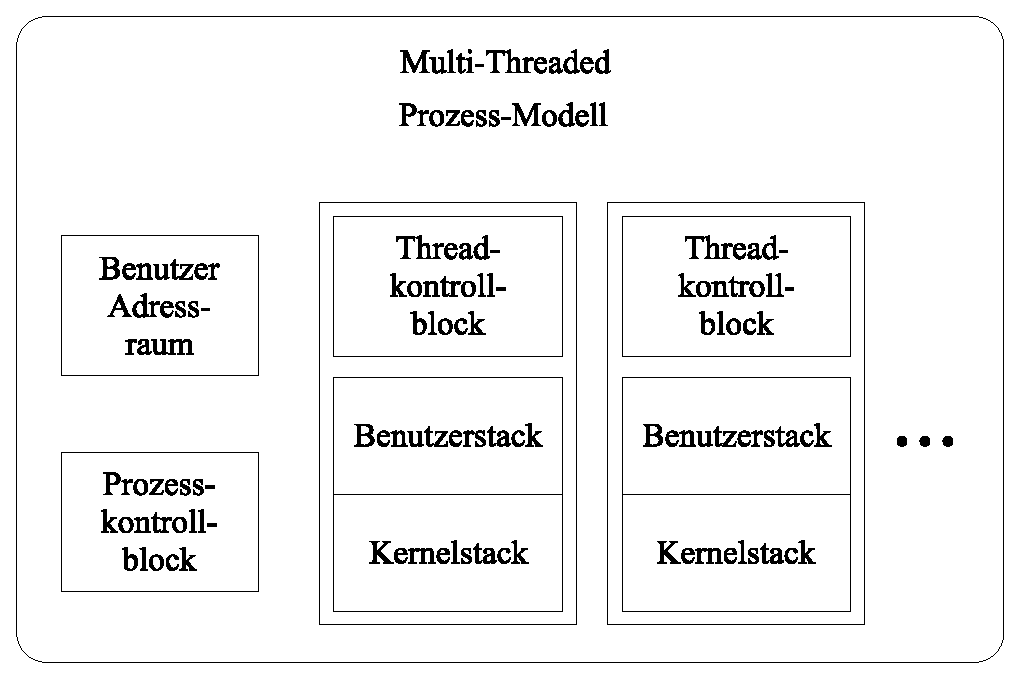
\includegraphics[width=10cm]{images/multithreadprozess.eps}
      \caption{Multi-Thread-Prozess-Modell}
      \label{fig:multithreadprozess}
    \end{figure}
    Der Interpreter CYBOI wird in C geschrieben. Dieser Quelltext wird unter Linux kompiliert 
    und ausgef�hrt. Eine M�glichkeit f�r Windows w�re \emph{cygwin}, das die kompletten GNU-Tools
    und Bibliotheken auch f�r Windows zur Verf�gung stellt. Die C-Bibliothek pthread 
    hat sich f�r die Threadbehandlung etabliert. In dieser Bibliothek sind M�glichkeiten zur 
    Erzeugung, Beendung und Synchronisation von Threads vorhanden.
     
  \subsection{Vergleich Threads und Prozesse}
   
    F�r die Integration des Webservers in CYBOI wurden die leichtgewichtigen Prozesse
    (Threads) ausgew�hlt. Da Threads innerhalb eines Prozesses von sich aus den gleichen Adressraum
    verwenden, ist eine direkte Kommunikation zwischen CYBOI und den Webserver �ber den
    gleichen Adressraum m�glich, womit bei Threads die Kommunikation �ber andere aufwendigere
    Kommunikationskan�le entf�llt. Ein weiterer Vorteil ist die Geschwindigkeit der Operationen von Threads.
    Da weniger Informationen involviert sind, sind die Operationen f�r Threads
    auch schneller als bei Prozessen. Dies betrifft sowohl die normalen Operationen, wie z.B. Aktivieren,
    Erzeugen, Blockieren als auch den Kontextwechsel zwischen den Threads. 
    Die Nachteile von Threads sind, dass dem Betriebssystem die Kontrolle �ber die Threads
    entzogen ist. Der Entwickler muss selbst darauf achten, dass sich diese nicht gegenseitig
    blockieren. Weiterhin ist durch die Benutzung des gleichen Adressraumes nicht der Schutz
    vor anderen Threads gesichert. Dieser ist ebenfalls vom Entwickler sicherzustellen. 
    
\section{Synchronisation von Threads}

  Die Kommunikation von Threads erfolgt �blichweise �ber den gemeinsamen 
  Benutzer-Adressraum. Da Threads nebenl�ufig arbeiten, m�ssen die Zugriffe auf gemeinsame Variablen 
  synchronisiert werden, da es ansonsten zu Kollisionen beim gleichzeitigen Zugriff 
  auf den gemeinsamen Speicherbereich kommen kann. Die pthread-Bibliothek stellt daf�r 
  zwei M�glichkeiten zur Verf�gung, entweder �ber Mutex oder mit Bedingungsvariablen.


  \subsection{Threadsynchronisation mit Mutex}

    Mutex ist ein Kunstwort, welches sich aus den W�rtern MUTual und EXclusions (gegenseitiger Ausschluss) 
    zusammensetzt. Sie dienen dazu, Ressourcen f�r Threads exklusiv zu reservieren. 
    Dabei kann ein Mutex immer nur von einem Thread belegt sein. Versuchen weitere Threads diesen Mutex f�r 
    sich zu beanspruchen, werden diese blockiert, bis der aktuelle Besitzer den Mutex wieder freigibt. 
    Da die Belegung atomar erfolgt, ist auch sichergestellt, dass immer nur ein Thread einen Mutex 
    zur selben Zeit belegt. Mutex liegt das Semaphoren-Konzept zu Grunde.
    
    Semaphor im Allgemeinen bedeutet, dass ein Zugriff auf einen kritischen Bereich (Shared memory) 
    gesch�tzt wird. Dazu besteht ein Semaphor aus zwei Elementen, dem Semaphor-Wert s(ganzzahlig) 
    und einer Warteschlange. Ist der Semaphoren-Wert gr��er Null, so bedeutet dies, 
    dass der kritische Abschnitt 
    betreten werden kann. Ansonsten ist der Abschnitt durch einen anderen Prozess belegt. 
    Die Warteschlange dient zur Speicherung aller Prozesse, die nicht den kritischen Abschnitt 
    betreten konnten.
    Zum weiteren sind f�r Semaphoren zwei Operationen P(s) und V(s) folgenderma�en definiert.
    \\ \\
    \verb|    P(s):  s = 0 | $\rightarrow$ Prozess in Warteschlange schlafen legen
    \\
    \verb|           s > 0 | $\rightarrow$ s um eins erniedrigen
    \\
    \verb|    V(s): | $\rightarrow$ s um eins erh�hen
    \\
    \verb|          | $\rightarrow$ falls Warteschlange nicht leer ist, so n�chsten Prozess aufwecken
    \\ \\
    Ein bin�rer Semaphore ist ein normaler Semaphor mit Initialisierung der 
    Semaphoren-Variable auf eins. Mutexe stellen bin�re Semaphoren dar, wobei die 
    Implementierung ohne die Warteschlange realisiert wurde.  
    
    Das Prinzip von Mutex ist einfach. Ein Thread arbeitet mit einer globalen oder 
    statischen Variable, die f�r allen anderen Threads w�hrend einer Operation 
    von einem Mutex blockiert 
    (gesperrt) wird. Ben�tigt der Thread diese Variable nicht mehr, gibt er diese frei.
    Durch das Setzen der Sperren im Programm liegt die Verantwortung einer 
    Verklemmungsfreiheit  beim Programmierer.
    Dadurch k�nnen aber bei unsauberer Programmierung Deadlocks auftreten, falls
    ein Thread die Sperrung nicht ordnungsgem�� freigibt oder es Ressourcen anfordert, 
    obwohl es schon Ressourcen bekommen hat.
     
  \subsection{Threads synchronisieren mit Bedingungsvariablen}
  
  
    Die Bedingungsvariablen dienen dazu, den Eintritt bestimmter Bedingungen abzuwarten 
    beziehungsweise deren Erf�llung anzuzeigen und k�nnen dazu genutzt werden
    Threads zu synchronisieren. Bedingungsvariablen sind an Mutexe gekoppelt um 
    sicherzustellen, dass die Bedingungen immer nur von einem Thread zu einer 
    Zeit ge�ndert werden k�nnen. 
    In der folgenden Abbildung ist das Prinzip der \emph{Condition Variable} zu erkennen.
    Dies ist aus dem Buch \cite{linuxprog} entnommen.
    \begin{figure}[H]
      \centering
        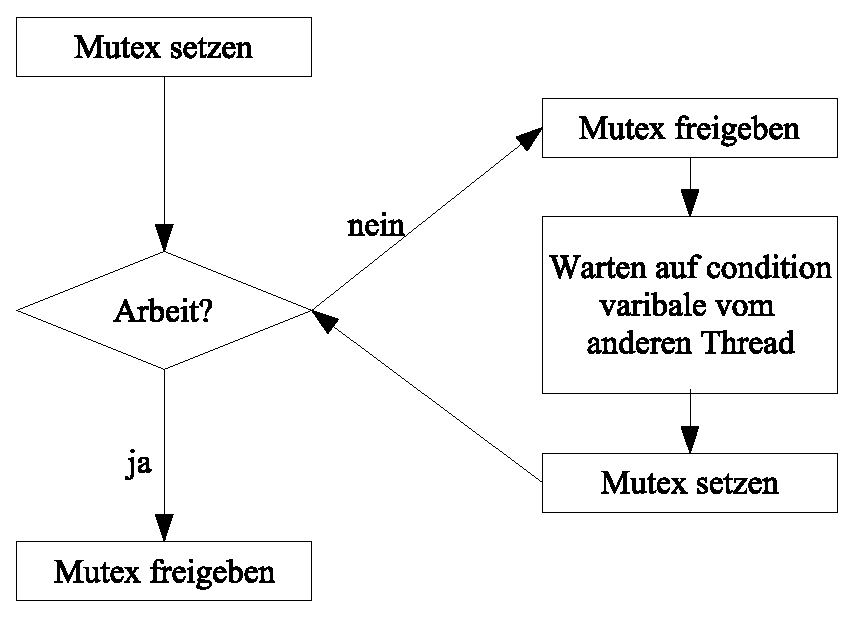
\includegraphics[width=10cm]{images/condvar.eps}
      \caption{Condition Variable}
      \label{fig:condvar}
    \end{figure}
    Am Anfang wird ein Mutex f�r einen kritischen Bereich gesetzt. Kann der Thread 
    nicht weiter arbeiten, weil zum Beispiel die ben�tigen Daten nicht anliegen, so
    wird dieser stillgelegt. Der Mutex wird freigegeben, es wird gewartet 
    bis diese Bedingung (Daten vorhanden) eintrifft und danach der Mutex wieder belegt. 
    Dies ist alles in einer Funktion der pthread-Bibliothek gekapselt. 
    Danach kann der Thread ganz normal seinen kritischen Bereich abarbeiten 
    und den Mutex wieder freigeben.

  \subsection{Fazit der Synchronisation}
  
    Die zwei vorgestellten Synchronisationsarten schlie�en sich nicht aus, sondern erg�nzen sich.
    Mutex ist f�r den einfachen gegenseitigen Ausschluss da. Dieser Mechanismus wird bei den 
    Bedingungsvariablen auch genutzt. Welche Form der Synchronisation ist f�r
    die Integration vom Webserver in CYBOI notwendig? Dazu ist die zu l�sende Aufgabe
    n�her zu betrachten. Wird im Webserver eine Anfrage vom Client gestellt, so ist ein Signal im
    \emph{Signal Memeory} zu erstellen. Dieses Signal ist die Umwandlung der Anfrage vom Client
    in die interne Repr�sentation von Signalen in CYBOI. Dazu ist es einfach nur notwendig, 
    die Variable \emph{Signal Memory} f�r den gegenseitigen Ausschluss zu sichern. Also ist 
    es ausreichend, die Synchronisation mit Mutex zu realisieren. 